\documentclass[11pt,spanish,a4paper]{article}
% Versión 1er cuat 2015 Víctor Bettachini < bettachini@df.uba.ar >

\usepackage{babel}
\addto\shorthandsspanish{\spanishdeactivate{~<>}}
\usepackage[utf8]{inputenc}
\usepackage{float}
\usepackage{units}
\usepackage{siunitx}
\usepackage{amsmath}
\usepackage{amstext}
\usepackage{amssymb}
\usepackage{graphicx}
\graphicspath{ {./graphs/} {../}}

\voffset-3.5cm
\hoffset-3cm
\setlength{\textwidth}{17.5cm}
\setlength{\textheight}{27cm}

\usepackage{lastpage}
\usepackage{fancyhdr}
\pagestyle{fancyplain}
\fancyhead{}
\fancyfoot{{\tiny \textcopyright Departamento de Física, FCEyN, UBA}}
\fancyfoot[C]{{\tiny Actualizado al \today}}
\fancyfoot[RO, LE]{Pág. \thepage/\pageref{LastPage}}
\renewcommand{\headrulewidth}{0pt}
\renewcommand{\footrulewidth}{0pt}


\begin{document}
\begin{center}
	\textsc{\large Física 2 (Físicos)} - Prof. Hernán Grecco - 1"er cuat. 2015\\
	\textsc{\large Guía 5:}	Ondas propagantes
\end{center}

\begin{enumerate}
\item Demuestre que la onda sinusoidal propagante es solución de la ecuación de Klein-Gordon.
	Grafique la relación de dispersión.
	Indique como se determina en ese gráfico la velocidad de fase.
	Calcule analíticamente la velocidad de fase y grafíquela.


\item Se tiene una cerda semi-infinita que se extiende hacia la izquierda.
	En \(x=L\) tiene su extremo.
	Una onda de amplitud A incide desde la izquierda.
	Calcule la expresión para la onda reflejada en este sistema de coordenadas.
	Repita el cálculo haciendo un cambio de variables de modo que el origen esté en el punto fijo, y vuelva a cambiar sobre el resultado al sistema original.
	Discuta como es la mecánica para este procedimiento.


\item Repita el problema anterior para una cuerda que cambia su densidad en \(x=L\).
	Calcule la onda reflejada y transmitida en ese sistema por los dos métodos.


\item Repita el problema anterior para el caso de una cuerda en la que se agrega una cuenta de masa \(m\) en \(x=L\).


\item Se tiene una cuerda de densidad lineal de masa \(\rho_1\) sometida a una tensión \(T_0\).
	A una distancia \(L\) del extremo la densidad lineal de la cuerda cambia abruptamente al valor \(\rho_2\) y a una distancia \(L+L'\) del mismo extremo el valor de \(\rho\) vuelve a ser \(\rho_1\).
	En esta cuerda se propaga una onda de la forma \(A \cos{(\omega t- k_1 z)}\).
	Escribir la forma de la función de onda (sin importar su amplitud) para las ondas transmitidas, y para los siguientes sistemas de referencia:
	\begin{enumerate}
		\item el origen de coordenadas en el extremo de la primer cuerda de densidad \(\rho_1\), 
		\item el origen de coordenadas en el primer punto de cambio de \(\rho\), 
		\item el origen de coordenadas en el segundo punto de cambio de \(\rho\).
	\end{enumerate}
\begin{center}
	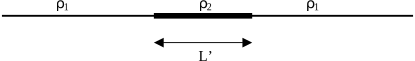
\includegraphics[width=0.45\linewidth]{g05e05}
\end{center}


\item Un resorte semi-infinito de constante distribuida \(K_i\) y densidad lineal \(\rho\) se extiende desde la izquierda hasta \(x=L\).
	Termina en un cuerpo de masa \(M\) como indica la figura.
	Encuentre el coeficiente de reflexión en función de la frecuencia y la masa \(M\).
	Discuta el resultado.
\begin{center}
	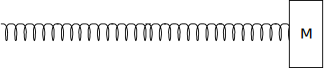
\includegraphics[width=0.45\linewidth]{g05e06}
\end{center}


\item Repita el problema anterior si la masa de terminación es remplazada por un amortiguador que
ejerce una fuerza sobre el resorte oponiéndose al movimiento y proporcional a la velocidad.
\begin{center}
	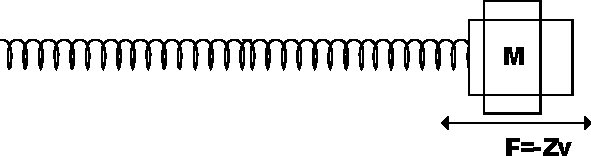
\includegraphics[width=0.45\linewidth]{g05e07}
\end{center}


\item  Se tienen dos resortes semi-infinitos de distinta densidad lineal de masa (\(\rho_1\) y \(\rho_2\)), y constantes \(K_{i1}\) y \(K_{i2}\) unidos en un punto.
	\begin{enumerate}
		\item Conocida \(\rho_1\) y \(K_{i1}\) calcule \(\rho_2\) y \(K_{i2}\) para que a la onda reflejada le corresponda una amplitud que sea la mitad de la amplitud de la onda incidente.
			Considere los dos casos de incidencia posibles (desde la izquierda y desde la derecha).
		\item Grafique los coeficientes de reflexión y de transmisión vs \(\rho_2\).
		\item Vea que para cualquier recinto que incluya o no a la unión el flujo de energía que entra es igual al flujo de energía que sale.
	\end{enumerate}


\item Se tiene el siguiente sistema, forzado en \(z=0\), tal que \(\psi(0,t)= A_o \cos{(t)}\).
	No tenga en cuenta el rozamiento.
	\begin{enumerate}
		\item Calcule \(\psi(z,t)\).
		\item Calcule la fuerza que hay que hacer en \(z=0\) para que la cuerda se mueva de esta manera.
			Vea que es de la forma \(f(t)= f_0 \cos{(t)}\).
			¿Cuál es la relación entre \(A_0\) y \(f_0\)?
			¿Cómo es \(\frac{\partial \psi}{\partial z}\) en \(z=0\)?
			¿En qué caso es continua?.
		\item Si en vez de conocer el vínculo en \(z=0\) (\(\psi(0,t)\)) se conoce la fuerza que se realiza sobre la cuerda en ese punto, y se sabe que dicha fuerza es de la forma \(f(t)= f_0 \cos{(t)}\), ¿cómo será el movimiento de la cuerda? (Use lo calculado en b)).
		\item En \(t=0\) se deja al sistema en libertad.
			Si la frecuencia de excitación era \(\omega_1= \frac{3 \pi v}{4 L}\), calcule qué modos estarán excitados para \(t>0\) y cuáles serán los más importantes.
			Dibuje \(\psi(z,0)\) y los modos más importantes.
			¿Es cierto que al liberar al sistema éste sigue oscilando con la frecuencia de excitación para \(t<0\)?
	\end{enumerate}
\begin{center}
	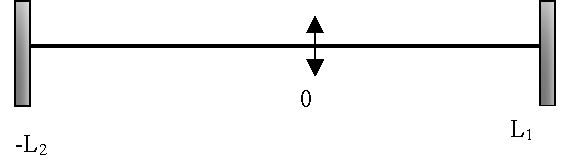
\includegraphics[width=0.45\linewidth]{g05e09}
\end{center}


\item Planteé el problema anterior en el caso en que se incluyen en la ecuación de ondas pérdidas
proporcionales a la velocidad.


\item Calcule los coeficientes de reflexión y de transmisión del sonido en las siguientes interfases:
	\begin{enumerate}
		\item hierro-cobre, 
		\item aluminio-plomo,
		\item aire-agua.
	\end{enumerate}


\item Un tubo lleno de aire tiene un parlante en un extremo y el otro abierto.
	¿Cómo son las condiciones de borde para calcular la amplitud de la onda sonora reflejada?
	¿Y si el tubo está abierto?


\end{enumerate}
\end{document}
